\documentclass[11pt,a4paper]{article}
\usepackage[top=2cm, bottom=2.5cm, left=1.8cm, right=1.8cm, headsep=0.8cm]{geometry}
\usepackage{amsmath,amssymb,amsfonts}
\usepackage{enumitem}
\usepackage{fancyhdr}
\usepackage{xcolor}
\usepackage{tcolorbox}
\usepackage{tabularx}
\usepackage{multicol}
\usepackage{tikz}
\usetikzlibrary{arrows.meta,patterns,calc}

% Color definitions
\definecolor{deepblue}{RGB}{20,45,110}
\definecolor{accentblue}{RGB}{41,128,185}
\definecolor{darkgray}{RGB}{50,50,50}
\definecolor{lightgray}{RGB}{245,247,250}
\definecolor{borderblue}{RGB}{200,215,235}

% Page styling
\pagestyle{fancy}
\fancyhf{}
\fancyhead[L]{\small\textsf{\textbf{JEE ADVANCED / MAIN TEST SERIES}}}
\fancyhead[C]{\small\textsf{\textcolor{accentblue}{PHYSICS: ROTATIONAL MOTION}}}
\fancyhead[R]{\small\textsf{MAX MARKS: 100}}
\fancyfoot[C]{\thepage}
\renewcommand{\headrulewidth}{0.6pt}
\renewcommand{\footrulewidth}{0.4pt}

% Custom boxes
\tcbset{
  testheader/.style={
    colback=lightgray,
    colframe=deepblue,
    boxrule=1.2pt,
    arc=4mm,
    left=15pt,right=15pt,top=10pt,bottom=10pt
  },
  sectionheader/.style={
    colback=deepblue,
    coltext=white,
    boxrule=0pt,
    arc=2mm,
    left=8pt,right=8pt,top=5pt,bottom=5pt
  },
  solbox/.style={
    colback=lightgray,
    colframe=borderblue,
    boxrule=0.8pt,
    arc=2mm,
    left=10pt,right=10pt,top=8pt,bottom=8pt
  }
}

\begin{document}

% ==================== HEADER BOX ====================
\begin{tcolorbox}[testheader]
\begin{center}
  {\LARGE \textbf{\textsf{\textcolor{deepblue}{STUDYFAM JEE PREPARATION SERIES}}}}\\[3pt]
  {\large \textbf{\textsf{TOPICAL TEST: ROTATIONAL MOTION}}}\\[6pt]
  {\small \textbf{Target:} JEE (Main + Advanced) \quad $\vert$ \quad \textbf{Total Questions:} 25 \quad $\vert$ \quad \textbf{Time:} 60 Minutes \quad $\vert$ \quad \textbf{Max. Marks:} 100}
\end{center}
\vspace{-4pt}
\hrule
\vspace{6pt}
\footnotesize
\textbf{Marking Scheme:}
\begin{itemize}[leftmargin=15pt,itemsep=1pt,topsep=1pt]
  \item \textbf{Section I (Single Correct Choice, Q1--Q20):} $+4$ for correct answer; $-1$ for incorrect answer; $0$ if unattempted.
  \item \textbf{Section II (Numerical Value, Q21--Q25):} $+4$ for correct numerical answer; $0$ for incorrect answer; $0$ if unattempted.
\end{itemize}
\end{tcolorbox}

\vspace{10pt}

% ==================== SECTION I ====================
\begin{tcolorbox}[sectionheader]
  \textbf{\textsf{SECTION I: SINGLE CORRECT CHOICE TYPE (20 Questions $\times$ 4 Marks = 80 Marks)}}
\end{tcolorbox}
\vspace{4pt}
\textit{Each question has four options (A), (B), (C), and (D). Exactly ONE of these four options is correct.}
\vspace{6pt}

\begin{enumerate}[label=\textbf{Q\arabic*.},leftmargin=24pt,itemsep=12pt]

  % Q1
  \item The moment of inertia of a rigid body does \textbf{NOT} depend upon:
  \begin{enumerate}[label=(\Alph*),itemsep=2pt]
    \item Distribution of mass about the axis of rotation
    \item Orientation and position of the axis of rotation
    \item Angular velocity of the body
    \item Total mass of the body
  \end{enumerate}

  % Q2
  \item The moment of inertia of a uniform circular wire (ring) of mass $M$ and radius $R$ about its diameter is:
  \begin{multicols}{2}
  \begin{enumerate}[label=(\Alph*),itemsep=2pt]
    \item $\dfrac{1}{2} M R^2$
    \item $M R^2$
    \item $\dfrac{1}{4} M R^2$
    \item $2 M R^2$
  \end{enumerate}
  \end{multicols}

  % Q3
  \item The moment of inertia of a thin hollow cylinder (cylindrical shell) of mass $M$ and radius $r$ about its own geometrical symmetry axis is:
  \begin{multicols}{2}
  \begin{enumerate}[label=(\Alph*),itemsep=2pt]
    \item $\dfrac{2}{3} M r^2$
    \item $\dfrac{2}{5} M r^2$
    \item $\dfrac{1}{2} M r^2$
    \item $M r^2$
  \end{enumerate}
  \end{multicols}

  % Q4
  \item The moment of inertia of a uniform circular disc of radius $R$ and mass $M$ about an axis passing through its edge (rim) and perpendicular to the plane of the disc is:
  \begin{multicols}{2}
  \begin{enumerate}[label=(\Alph*),itemsep=2pt]
    \item $M R^2$
    \item $\dfrac{1}{2} M R^2$
    \item $\dfrac{3}{2} M R^2$
    \item $\dfrac{7}{2} M R^2$
  \end{enumerate}
  \end{multicols}

  % Q5
  \item Point masses of $1\text{ kg}$, $2\text{ kg}$, $3\text{ kg}$, and $4\text{ kg}$ are lying at points $(0, 0, 0)$, $(2, 0, 0)$, $(0, 3, 0)$, and $(-2, -2, 0)$ respectively in the $xy$-plane (all coordinates in meters). The moment of inertia of this system about the $x$-axis is:
  \begin{multicols}{2}
  \begin{enumerate}[label=(\Alph*),itemsep=2pt]
    \item $43\text{ kg}\cdot\text{m}^2$
    \item $34\text{ kg}\cdot\text{m}^2$
    \item $27\text{ kg}\cdot\text{m}^2$
    \item $72\text{ kg}\cdot\text{m}^2$
  \end{enumerate}
  \end{multicols}

  % Q6
  \item From a solid sphere of uniform mass density, mass $M$, and radius $R$, a cube of the maximum possible volume is cut out. The moment of inertia of this cube about an axis passing through its center of mass and perpendicular to one of its faces is:
  \begin{multicols}{2}
  \begin{enumerate}[label=(\Alph*),itemsep=2pt]
    \item $\dfrac{4 M R^2}{9\sqrt{3}\pi}$
    \item $\dfrac{4 M R^2}{3\sqrt{3}\pi}$
    \item $\dfrac{M R^2}{32\sqrt{2}\pi}$
    \item $\dfrac{M R^2}{16\sqrt{2}\pi}$
  \end{enumerate}
  \end{multicols}

  % Q7
  \item A thin uniform rod of mass $M$ and length $L$ is rotated about an axis passing through its center and inclined at an angle $\theta$ to the length of the rod. The moment of inertia of the rod about this axis is:
  \begin{multicols}{2}
  \begin{enumerate}[label=(\Alph*),itemsep=2pt]
    \item $\dfrac{M L^2 \cos\theta}{12}$
    \item $\dfrac{M L^2 \sin^2\theta}{12}$
    \item $\dfrac{M L^2 \cos^2\theta}{18}$
    \item $\dfrac{M L^2 \sin^2\theta}{18}$
  \end{enumerate}
  \end{multicols}

  % Q8
  \item The radius of gyration $K$ of a hollow sphere of mass $M$ and radius $R$ about a certain axis is equal to $R$. The distance of that axis from the center of the sphere is:
  \begin{multicols}{2}
  \begin{enumerate}[label=(\Alph*),itemsep=2pt]
    \item $\dfrac{R}{\sqrt{2}}$
    \item $\dfrac{R}{\sqrt{3}}$
    \item $\dfrac{R}{\sqrt{7}}$
    \item $\dfrac{R}{\sqrt{5}}$
  \end{enumerate}
  \end{multicols}

  % Q9
  \item A wheel having an angular momentum of $2\pi\text{ kg}\cdot\text{m}^2/\text{s}$ about its vertical axis rotates at the rate of $60\text{ rpm}$ about this axis. The constant braking torque which can stop the wheel's rotation in $30\text{ s}$ is:
  \begin{multicols}{2}
  \begin{enumerate}[label=(\Alph*),itemsep=2pt]
    \item $\dfrac{2\pi}{15}\text{ N}\cdot\text{m}$
    \item $\dfrac{\pi}{18}\text{ N}\cdot\text{m}$
    \item $\dfrac{\pi}{12}\text{ N}\cdot\text{m}$
    \item $\dfrac{\pi}{15}\text{ N}\cdot\text{m}$
  \end{enumerate}
  \end{multicols}

  % Q10
  \item A couple acting on a rigid body produces:
  \begin{enumerate}[label=(\Alph*),itemsep=2pt]
    \item Purely linear (translational) motion
    \item Purely rotational motion
    \item Combined linear and rotational motion
    \item No motion under any circumstances
  \end{enumerate}

  % Q11
  \item A ball rolls without slipping on a horizontal plane. The radius of gyration of the ball about an axis passing through its center of mass is $K$. If the radius of the ball is $R$, then the fraction of its total kinetic energy associated with rotational motion is:
  \begin{multicols}{2}
  \begin{enumerate}[label=(\Alph*),itemsep=2pt]
    \item $\dfrac{K^2}{R^2}$
    \item $\dfrac{K^2}{K^2 + R^2}$
    \item $\dfrac{R^2}{K^2 + R^2}$
    \item $\dfrac{K^2 + R^2}{R^2}$
  \end{enumerate}
  \end{multicols}

  % Q12
  \item A wheel of radius $R = 1\text{ m}$ rolls forward through half a revolution without slipping on a horizontal ground. The magnitude of the net displacement of the point on the wheel initially in contact with the ground is:
  \begin{multicols}{2}
  \begin{enumerate}[label=(\Alph*),itemsep=2pt]
    \item $\pi\text{ m}$
    \item $2\pi\text{ m}$
    \item $\sqrt{\pi^2 + 9}\text{ m}$
    \item $\sqrt{\pi^2 + 4}\text{ m}$
  \end{enumerate}
  \end{multicols}

  % Q13
  \item A flywheel rotating about a fixed axis has a kinetic energy of $360\text{ J}$ when its angular speed is $30\text{ rad/s}$. The moment of inertia of the wheel about the axis of rotation is:
  \begin{multicols}{2}
  \begin{enumerate}[label=(\Alph*),itemsep=2pt]
    \item $0.6\text{ kg}\cdot\text{m}^2$
    \item $0.15\text{ kg}\cdot\text{m}^2$
    \item $0.8\text{ kg}\cdot\text{m}^2$
    \item $0.75\text{ kg}\cdot\text{m}^2$
  \end{enumerate}
  \end{multicols}

  % Q14
  \item A bullet of mass $10\text{ g}$ moving with speed $500\text{ m/s}$ is fired horizontally into a uniform door and gets embedded exactly at the center of the door. The door has width $w = 1.0\text{ m}$ and mass $M = 12\text{ kg}$, and is hinged along one vertical edge so it can rotate practically without friction. The angular speed of the door immediately after the bullet embeds into it is:
  \begin{multicols}{2}
  \begin{enumerate}[label=(\Alph*),itemsep=2pt]
    \item $6.25\text{ rad/s}$
    \item $0.625\text{ rad/s}$
    \item $3.35\text{ rad/s}$
    \item $0.335\text{ rad/s}$
  \end{enumerate}
  \end{multicols}

  % Q15
  \item When a ceiling fan is switched off, its angular velocity falls to half of its initial value while it makes $36$ complete rotations. Assuming a uniform angular retardation, how many more rotations will it make before coming to rest?
  \begin{multicols}{2}
  \begin{enumerate}[label=(\Alph*),itemsep=2pt]
    \item $24$
    \item $36$
    \item $18$
    \item $12$
  \end{enumerate}
  \end{multicols}

  % Q16
  \item A thin hoop of radius $r$ and mass $m$ rotating with an angular velocity $\omega_0$ about its central axis is placed gently on a rough horizontal surface. The initial translational velocity of the center of mass is zero. What will be the linear velocity of the center of the hoop when it ceases to slip and starts pure rolling?
  \begin{multicols}{2}
  \begin{enumerate}[label=(\Alph*),itemsep=2pt]
    \item $\dfrac{r\omega_0}{4}$
    \item $\dfrac{r\omega_0}{3}$
    \item $\dfrac{r\omega_0}{2}$
    \item $r\omega_0$
  \end{enumerate}
  \end{multicols}

  % Q17
  \item A thin ring of mass $M$ and radius $R$ is rotating about its central perpendicular axis with angular velocity $\omega$. Two identical small bodies, each of mass $m$, are gently attached to the ring at the two opposite ends of a diameter. Because of this, the loss in rotational kinetic energy of the system is:
  \begin{multicols}{2}
  \begin{enumerate}[label=(\Alph*),itemsep=2pt]
    \item $\dfrac{m(M+2m)}{M}\omega^2 R^2$
    \item $\dfrac{Mm}{M+m}\omega^2 R^2$
    \item $\dfrac{Mm}{M+2m}\omega^2 R^2$
    \item $\dfrac{M(M+m)}{M+2m}\omega^2 R^2$
  \end{enumerate}
  \end{multicols}

  % Q18
  \item A uniform solid cylinder of mass $m$ and radius $R$ rolls down an inclined plane of vertical height $h$ from rest without slipping. The linear speed of its center of mass when it reaches the bottom of the incline is:
  \begin{multicols}{2}
  \begin{enumerate}[label=(\Alph*),itemsep=2pt]
    \item $\sqrt{2gh}$
    \item $\sqrt{\dfrac{4gh}{3}}$
    \item $\sqrt{\dfrac{3gh}{4}}$
    \item $\sqrt{4gh}$
  \end{enumerate}
  \end{multicols}

  % Q19
  \item If the angular momentum of a particle of mass $m$ rotating along a circular path of radius $r$ with uniform speed is $L$, the centripetal force acting on the particle is:
  \begin{multicols}{2}
  \begin{enumerate}[label=(\Alph*),itemsep=2pt]
    \item $\dfrac{L^2}{m r^3}$
    \item $\dfrac{L^2}{m r}$
    \item $\dfrac{L}{m r}$
    \item $\dfrac{L^2 m}{r}$
  \end{enumerate}
  \end{multicols}

  % Q20
  \item A solid sphere, a uniform circular disc, and a solid cylinder, all having the same mass and same radius, are released from rest from the same height on a rough inclined plane and roll down without slipping. Which of the following statements is correct?
  \begin{enumerate}[label=(\Alph*),itemsep=2pt]
    \item The solid sphere reaches the bottom first
    \item The solid sphere reaches the bottom last
    \item The disc reaches the bottom first
    \item All reach the bottom at the same time
  \end{enumerate}

\end{enumerate}

\vspace{15pt}

% ==================== SECTION II ====================
\begin{tcolorbox}[sectionheader]
  \textbf{\textsf{SECTION II: NUMERICAL VALUE TYPE (5 Questions $\times$ 4 Marks = 20 Marks)}}
\end{tcolorbox}
\vspace{4pt}
\textit{The answer to each of the following questions is a non-negative numerical value. Enter the exact integer or decimal value.}
\vspace{6pt}

\begin{enumerate}[label=\textbf{Q\arabic*.},leftmargin=24pt,itemsep=16pt,start=21]

  % Q21 (DB Q30)
  \item A wheel of radius $R = 1\text{ m}$ is rolling without sliding uniformly on a horizontal surface. Find the radius of curvature (in $\text{m}$) of the path of a point on its circumference when it reaches the highest point in its cycloidal path.

  % Q22 (DB Q27)
  \item A uniform rod $AB$ of mass $M = 2\text{ kg}$ and length $L$ is hinged at one end $A$ to a vertical wall. The rod is held in the horizontal position by a light vertical string tied to the end $B$. At $t = 0$, the string at $B$ is cut. Determine the reaction force exerted by the hinge (in $\text{N}$) on end $A$ of the rod at the instant immediately after the string is cut. (Take $g = 10\text{ m/s}^2$).
  
  \begin{center}
  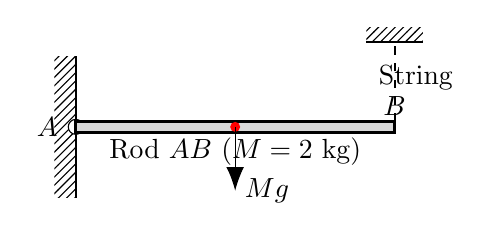
\begin{tikzpicture}[scale=0.9]
    % Wall
    \fill[pattern=north east lines] (-0.3,-1) rectangle (0,1);
    \draw[thick] (0,-1) -- (0,1);
    % Hinge at A
    \draw[fill=white] (0,0) circle (3pt) node[left=3pt] {$A$};
    % Rod AB
    \draw[very thick, fill=gray!30] (0,-0.08) rectangle (4.5,0.08);
    \node at (4.5,0.3) {$B$};
    \node at (2.25,-0.35) {Rod $AB$ ($M=2\text{ kg}$)};
    % Center of mass
    \fill[red] (2.25,0) circle (2pt);
    \draw[-{Latex[length=3mm]}] (2.25,0) -- (2.25,-0.9) node[right] {$Mg$};
    % String at B
    \draw[dashed, thick] (4.5,0.08) -- (4.5,1.2);
    \fill[pattern=north east lines] (4.1,1.2) rectangle (4.9,1.4);
    \draw[thick] (4.1,1.2) -- (4.9,1.2);
    \node at (4.8,0.7) {String};
  \end{tikzpicture}
  \end{center}

  % Q23 (DB Q28)
  \item A uniform solid cylinder of mass $M$, diameter $d = 4\text{ cm}$, and height $h = 10\text{ cm}$ rests upright on a flat horizontal cart. The coefficient of static friction between the cylinder and the cart is $\mu = 0.5$. Find the minimum horizontal acceleration (in $\text{m/s}^2$) of the cart needed to cause the cylinder to tip over without sliding. (Take $g = 10\text{ m/s}^2$).
  
  \begin{center}
  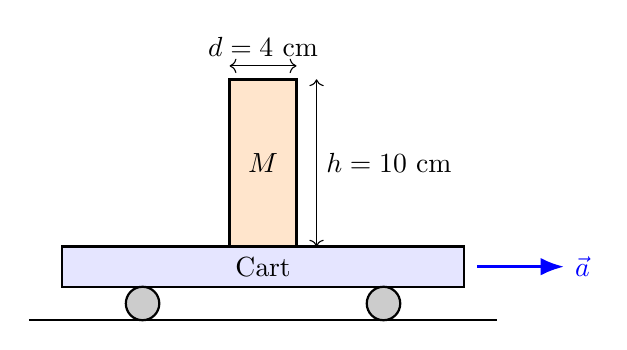
\begin{tikzpicture}[scale=0.85]
    % Cart
    \draw[thick, fill=blue!10] (0,0) rectangle (6,0.6);
    \draw[thick, fill=gray!40] (1.2,-0.25) circle (0.25);
    \draw[thick, fill=gray!40] (4.8,-0.25) circle (0.25);
    \draw[thick] (-0.5,-0.5) -- (6.5,-0.5);
    \draw[-{Latex[length=3mm]}, very thick, blue] (6.2,0.3) -- (7.5,0.3) node[right] {$\vec{a}$};
    % Cylinder
    \draw[very thick, fill=orange!20] (2.5,0.6) rectangle (3.5,3.1);
    \node at (3,1.85) {$M$};
    % Dimensions
    \draw[<->] (2.5,3.3) -- (3.5,3.3) node[midway,above] {$d = 4\text{ cm}$};
    \draw[<->] (3.8,0.6) -- (3.8,3.1) node[midway,right] {$h = 10\text{ cm}$};
    \node at (3,0.3) {Cart};
  \end{tikzpicture}
  \end{center}

  % Q24 (DB Q22)
  \item A light (weightless) rigid rod of length $l$ with a small concentrated load of mass $m$ fixed at its upper end is hinged at point $A$ on a smooth horizontal floor. The rod initially stands in a strictly vertical position, touching a block of mass $M$ placed on the floor. A slight jerk sets the system into motion. Find the mass ratio $M/m$ such that the rod forms an angle $\theta = \dfrac{\pi}{6}$ ($30^\circ$) with the horizontal floor at the instant the small mass separates from the block.
  
  \begin{center}
  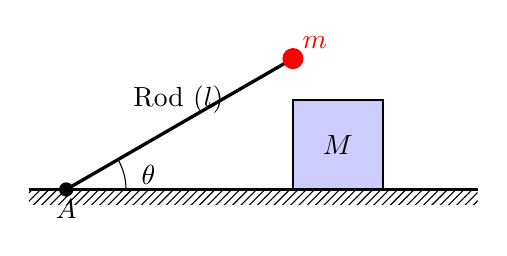
\begin{tikzpicture}[scale=0.95]
    % Floor
    \fill[pattern=north east lines] (-0.5,-0.2) rectangle (5.5,0);
    \draw[thick] (-0.5,0) -- (5.5,0);
    % Hinge A
    \draw[fill=black] (0,0) circle (2.5pt) node[below] {$A$};
    % Rod at angle theta
    \draw[very thick] (0,0) -- ({3.5*cos(30)},{3.5*sin(30)});
    % Mass m at end
    \fill[red] ({3.5*cos(30)},{3.5*sin(30)}) circle (4pt) node[above right] {$m$};
    % Angle theta
    \draw (0.8,0) arc (0:30:0.8);
    \node at (1.1,0.2) {$\theta$};
    % Block M
    \draw[thick, fill=blue!20] ({3.5*cos(30)},0) rectangle ({3.5*cos(30)+1.2},1.2);
    \node at ({3.5*cos(30)+0.6},0.6) {$M$};
    \node at (1.5,1.2) {Rod ($l$)};
  \end{tikzpicture}
  \end{center}

  % Q25 (DB Q25)
  \item A uniform solid cylinder of mass $M = 9\text{ kg}$ is at rest on a fixed rough plane inclined at an angle $\theta = 37^\circ$ with the horizontal. A light string wrapped around the cylinder passes horizontally to an ideal pulley and supports a hanging block of mass $m$, as shown. If the system remains in static equilibrium without slipping, find the mass $m$ of the hanging block (in $\text{kg}$). (Take $\sin 37^\circ = 0.6$, $\cos 37^\circ = 0.8$, $g = 10\text{ m/s}^2$).
  
  \begin{center}
  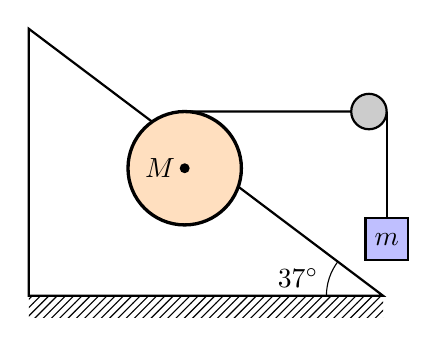
\begin{tikzpicture}[scale=0.9]
    % Incline
    \draw[thick] (0,0) -- (5,0) -- (0,{5*tan(37)}) -- cycle;
    \fill[pattern=north east lines] (0,0) -- (5,0) -- (5,-0.3) -- (0,-0.3) -- cycle;
    \draw (4.2,0) arc (180:143:0.8);
    \node at (3.8,0.25) {$37^\circ$};
    % Cylinder on incline
    \coordinate (C) at (2.2, 1.8);
    \draw[very thick, fill=orange!25] (C) circle (0.8);
    \fill (C) circle (2pt) node[left] {$M$};
    % String from top of cylinder
    \coordinate (T) at ($(C)+(0,0.8)$);
    \draw[thick] (T) -- (4.8, 2.6);
    % Pulley
    \draw[thick, fill=gray!40] (4.8, 2.6) circle (0.25);
    % Hanging string and mass
    \draw[thick] (5.05, 2.6) -- (5.05, 1.1);
    \draw[thick, fill=blue!25] (4.75, 0.5) rectangle (5.35, 1.1);
    \node at (5.05, 0.8) {$m$};
  \end{tikzpicture}
  \end{center}

\end{enumerate}

\newpage

% ==================== ANSWER KEY ====================
\begin{tcolorbox}[sectionheader]
  \textbf{\textsf{ANSWER KEY}}
\end{tcolorbox}
\vspace{6pt}

\begin{center}
\renewcommand{\arraystretch}{1.3}
\begin{tabular}{|c|c||c|c||c|c||c|c||c|c|}
\hline
\textbf{Q.} & \textbf{Ans.} & \textbf{Q.} & \textbf{Ans.} & \textbf{Q.} & \textbf{Ans.} & \textbf{Q.} & \textbf{Ans.} & \textbf{Q.} & \textbf{Ans.} \\
\hline\hline
1 & \textbf{C} & 6 & \textbf{A} & 11 & \textbf{B} & 16 & \textbf{C} & 21 & \textbf{4} \\
\hline
2 & \textbf{A} & 7 & \textbf{B} & 12 & \textbf{D} & 17 & \textbf{C} & 22 & \textbf{5} \\
\hline
3 & \textbf{D} & 8 & \textbf{B} & 13 & \textbf{C} & 18 & \textbf{B} & 23 & \textbf{4} \\
\hline
4 & \textbf{C} & 9 & \textbf{D} & 14 & \textbf{B} & 19 & \textbf{A} & 24 & \textbf{4} \\
\hline
5 & \textbf{A} & 10 & \textbf{B} & 15 & \textbf{D} & 20 & \textbf{A} & 25 & \textbf{3} \\
\hline
\end{tabular}
\end{center}

\vspace{15pt}

% ==================== STEP-BY-STEP SOLUTIONS ====================
\begin{tcolorbox}[sectionheader]
  \textbf{\textsf{HINTS AND STEP-BY-STEP SOLUTIONS}}
\end{tcolorbox}
\vspace{8pt}

\subsection*{Section I: Single Correct Choice}

\begin{enumerate}[label=\textbf{Q\arabic*.},leftmargin=24pt,itemsep=10pt]

  \item \textbf{Correct Option: (C)}\\
  \textit{Explanation:} The moment of inertia $I = \sum m_i r_i^2 = \int r^2 dm$ depends purely on the mass, the shape/dimensions of the body, the mass distribution, and the position and orientation of the axis of rotation. It does \textbf{not} depend on the kinematic state of motion such as angular velocity $\omega$ or angular acceleration $\alpha$.

  \item \textbf{Correct Option: (A)}\\
  \textit{Explanation:} For a planar circular ring lying in the $xy$-plane, by perpendicular axis theorem:
  \[
    I_z = I_x + I_y
  \]
  By circular symmetry, the moment of inertia about any diameter is identical: $I_x = I_y = I_d$.
  \[
    I_z = M R^2 \implies 2 I_d = M R^2 \implies I_d = \frac{1}{2} M R^2
  \]

  \item \textbf{Correct Option: (D)}\\
  \textit{Explanation:} In a thin hollow cylinder (cylindrical shell) of radius $r$, every single mass element $dm$ is at the exact same radial distance $r$ from the central longitudinal symmetry axis. Hence:
  \[
    I = \int r^2 dm = r^2 \int dm = M r^2
  \]

  \item \textbf{Correct Option: (C)}\\
  \textit{Explanation:} The moment of inertia of a uniform disc about an axis passing through its center of mass perpendicular to its plane is $I_{\text{cm}} = \frac{1}{2} M R^2$. Using the parallel axis theorem for an axis along the edge at distance $d = R$:
  \[
    I = I_{\text{cm}} + M d^2 = \frac{1}{2} M R^2 + M R^2 = \frac{3}{2} M R^2
  \]

  \item \textbf{Correct Option: (A)}\\
  \textit{Explanation:} The moment of inertia of a system of particles about the $x$-axis depends on the perpendicular distance of each mass from the $x$-axis, which is its $y$-coordinate ($r_{i,\perp} = |y_i|$):
  \[
    I_x = \sum_{i=1}^4 m_i y_i^2 = 1(0)^2 + 2(0)^2 + 3(3)^2 + 4(-2)^2 = 0 + 0 + 27 + 16 = 43\text{ kg}\cdot\text{m}^2
  \]

  \item \textbf{Correct Option: (A)}\\
  \textit{Explanation:} A cube inscribed in a sphere of radius $R$ has its main body diagonal equal to the diameter of the sphere:
  \[
    \sqrt{3} a = 2R \implies a = \frac{2R}{\sqrt{3}}
  \]
  The volume of the sphere is $V_{\text{sphere}} = \frac{4}{3}\pi R^3$, so its uniform density is $\rho = \frac{M}{\frac{4}{3}\pi R^3} = \frac{3M}{4\pi R^3}$.\\
  The mass of the cut-out cube is:
  \[
    M' = \rho a^3 = \left(\frac{3M}{4\pi R^3}\right) \left(\frac{2R}{\sqrt{3}}\right)^3 = \frac{3M}{4\pi R^3} \frac{8 R^3}{3\sqrt{3}} = \frac{2M}{\sqrt{3}\pi}
  \]
  The moment of inertia of a uniform cube of mass $M'$ and side $a$ about an axis through its center perpendicular to a face is $I = \frac{1}{6} M' a^2$:
  \[
    I = \frac{1}{6} \left(\frac{2M}{\sqrt{3}\pi}\right) \left(\frac{4 R^2}{3}\right) = \frac{4 M R^2}{9\sqrt{3}\pi}
  \]

  \item \textbf{Correct Option: (B)}\\
  \textit{Explanation:} Consider a mass element $dm = \frac{M}{L} dx$ located at distance $x$ from the center of the rod along its length. The perpendicular distance from this element to the axis inclined at angle $\theta$ is $r_\perp = x \sin\theta$.
  \[
    I = \int_{-L/2}^{L/2} r_\perp^2 dm = \int_{-L/2}^{L/2} (x \sin\theta)^2 \left(\frac{M}{L}\right) dx = \frac{M \sin^2\theta}{L} \left[ \frac{x^3}{3} \right]_{-L/2}^{L/2} = \frac{M L^2 \sin^2\theta}{12}
  \]

  \item \textbf{Correct Option: (B)}\\
  \textit{Explanation:} For a hollow spherical shell, $I_{\text{cm}} = \frac{2}{3} M R^2$. Let $d$ be the distance of the parallel axis from the center. By the parallel axis theorem:
  \[
    I = I_{\text{cm}} + M d^2 = \frac{2}{3} M R^2 + M d^2
  \]
  Since the radius of gyration is $K = R$, $I = M K^2 = M R^2$:
  \[
    \frac{2}{3} M R^2 + M d^2 = M R^2 \implies M d^2 = \frac{1}{3} M R^2 \implies d = \frac{R}{\sqrt{3}}
  \]

  \item \textbf{Correct Option: (D)}\\
  \textit{Explanation:} The torque required to change angular momentum is given by:
  \[
    \tau = \left| \frac{\Delta L}{\Delta t} \right| = \frac{L_i - L_f}{\Delta t} = \frac{2\pi - 0}{30} = \frac{\pi}{15}\text{ N}\cdot\text{m}
  \]

  \item \textbf{Correct Option: (B)}\\
  \textit{Explanation:} A couple consists of two equal and opposite parallel forces whose lines of action do not coincide. The net external force is $\sum \vec{F} = \vec{F} + (-\vec{F}) = 0$, so the acceleration of the center of mass is zero ($a_{\text{cm}} = 0$). Hence, a couple produces \textbf{purely rotational motion}.

  \item \textbf{Correct Option: (B)}\\
  \textit{Explanation:} For pure rolling ($v = \omega R$):
  \[
    K_{\text{rot}} = \frac{1}{2} I \omega^2 = \frac{1}{2} (M K^2) \left(\frac{v}{R}\right)^2 = \frac{1}{2} M v^2 \left(\frac{K^2}{R^2}\right)
  \]
  \[
    K_{\text{total}} = K_{\text{trans}} + K_{\text{rot}} = \frac{1}{2} M v^2 + \frac{1}{2} M v^2 \left(\frac{K^2}{R^2}\right) = \frac{1}{2} M v^2 \left(1 + \frac{K^2}{R^2}\right)
  \]
  The fraction of rotational kinetic energy is:
  \[
    \frac{K_{\text{rot}}}{K_{\text{total}}} = \frac{\frac{K^2}{R^2}}{1 + \frac{K^2}{R^2}} = \frac{K^2}{K^2 + R^2}
  \]

  \item \textbf{Correct Option: (D)}\\
  \textit{Explanation:} During half a revolution, the wheel rolls horizontally by a distance $\Delta x = \pi R = \pi(1) = \pi\text{ m}$. The contact point moves from the bottom ($y = 0$) to the top ($y = 2R = 2\text{ m}$).\\
  The net displacement vector is $\Delta \vec{r} = \pi \hat{i} + 2 \hat{j}$.
  \[
    |\Delta \vec{r}| = \sqrt{(\pi)^2 + (2)^2} = \sqrt{\pi^2 + 4}\text{ m}
  \]

  \item \textbf{Correct Option: (C)}\\
  \textit{Explanation:} Rotational kinetic energy is $K = \frac{1}{2} I \omega^2$.
  \[
    360 = \frac{1}{2} I (30)^2 = 450 I \implies I = \frac{360}{450} = 0.8\text{ kg}\cdot\text{m}^2
  \]

  \item \textbf{Correct Option: (B)}\\
  \textit{Explanation:} Angular momentum about the vertical hinge line is conserved during the rapid impact. Initial angular momentum:
  \[
    L_i = m v \left(\frac{w}{2}\right) = (0.01)(500)(0.5) = 2.5\text{ kg}\cdot\text{m}^2/\text{s}
  \]
  The moment of inertia of the door about its hinge is:
  \[
    I_{\text{door}} = \frac{1}{3} M w^2 = \frac{1}{3}(12)(1.0)^2 = 4\text{ kg}\cdot\text{m}^2
  \]
  (The bullet's contribution $m(w/2)^2 = 0.01(0.25) = 0.0025\text{ kg}\cdot\text{m}^2$ is negligible).
  \[
    \omega = \frac{L_i}{I} = \frac{2.5}{4} = 0.625\text{ rad/s}
  \]

  \item \textbf{Correct Option: (D)}\\
  \textit{Explanation:} Using the rotational kinematic equation $\omega^2 = \omega_0^2 - 2\alpha \theta$:
  \[
    \left(\frac{\omega_0}{2}\right)^2 = \omega_0^2 - 2\alpha (36) \implies 72 \alpha = \frac{3}{4} \omega_0^2 \implies 2\alpha = \frac{\omega_0^2}{48}
  \]
  Let $n$ be the number of additional rotations until the fan comes to rest ($0 = \omega_1^2 - 2\alpha n$):
  \[
    0 = \left(\frac{\omega_0}{2}\right)^2 - 2\alpha n \implies 2\alpha n = \frac{\omega_0^2}{4} \implies n = \frac{\omega_0^2/4}{\omega_0^2/48} = 12\text{ rotations}
  \]

  \item \textbf{Correct Option: (C)}\\
  \textit{Explanation:} Kinetic friction provides torque about the center of mass to decrease angular speed, while accelerating the center of mass forward. Since friction acts along the ground, the net torque about any fixed point on the ground level is zero!\\
  Conserving angular momentum about a point on the ground surface:
  \[
    L_i = I_{\text{cm}} \omega_0 = (m r^2) \omega_0
  \]
  When pure rolling begins, $v = r\omega$:
  \[
    L_f = I_{\text{cm}} \omega + m v r = (m r^2) \omega + m (r\omega) r = 2 m r^2 \omega = 2 m r v
  \]
  Equating $L_i = L_f$:
  \[
    m r^2 \omega_0 = 2 m r v \implies v = \frac{r \omega_0}{2}
  \]

  \item \textbf{Correct Option: (C)}\\
  \textit{Explanation:} Initial moment of inertia $I_i = M R^2$. Initial angular momentum $L = M R^2 \omega$. Initial kinetic energy $K_i = \frac{L^2}{2 I_i} = \frac{1}{2} M R^2 \omega^2$.\\
  When two point masses $m$ are attached at the ends of a diameter, each is at distance $R$ from the center:
  \[
    I_f = M R^2 + 2(m R^2) = (M + 2m) R^2
  \]
  By conservation of angular momentum, the final kinetic energy is $K_f = \frac{L^2}{2 I_f}$.\\
  Loss in kinetic energy:
  \[
    \Delta K = K_i - K_f = \frac{L^2}{2} \left( \frac{1}{I_i} - \frac{1}{I_f} \right) = \frac{(M R^2 \omega)^2}{2} \left( \frac{2m R^2}{M R^2 (M + 2m) R^2} \right) = \frac{M m}{M + 2m} \omega^2 R^2
  \]

  \item \textbf{Correct Option: (B)}\\
  \textit{Explanation:} By conservation of mechanical energy for pure rolling down an incline of height $h$:
  \[
    mgh = \frac{1}{2} m v^2 + \frac{1}{2} I \omega^2
  \]
  For a solid cylinder, $I = \frac{1}{2} m R^2$ and $\omega = v/R$:
  \[
    mgh = \frac{1}{2} m v^2 + \frac{1}{4} m v^2 = \frac{3}{4} m v^2 \implies v = \sqrt{\frac{4gh}{3}}
  \]

  \item \textbf{Correct Option: (A)}\\
  \textit{Explanation:} The angular momentum of a particle in circular motion is $L = m v r \implies v = \frac{L}{m r}$. The centripetal force is:
  \[
    F_c = \frac{m v^2}{r} = \frac{m}{r} \left( \frac{L}{m r} \right)^2 = \frac{L^2}{m r^3}
  \]

  \item \textbf{Correct Option: (A)}\\
  \textit{Explanation:} The linear acceleration of a body rolling down an incline of angle $\theta$ is:
  \[
    a = \frac{g \sin\theta}{1 + \frac{I_{\text{cm}}}{m R^2}}
  \]
  \begin{itemize}
    \item Solid sphere: $\frac{I}{m R^2} = \frac{2}{5} = 0.4 \implies a = \frac{g \sin\theta}{1.4} = \frac{5}{7} g \sin\theta \approx 0.714 g \sin\theta$
    \item Disc / Solid cylinder: $\frac{I}{m R^2} = \frac{1}{2} = 0.5 \implies a = \frac{g \sin\theta}{1.5} = \frac{2}{3} g \sin\theta \approx 0.667 g \sin\theta$
  \end{itemize}
  Since the solid sphere has the smallest $\frac{I}{m R^2}$, it experiences the highest acceleration and therefore reaches the bottom in the shortest time.

\end{enumerate}

\subsection*{Section II: Numerical Value Type}

\begin{enumerate}[label=\textbf{Q\arabic*.},leftmargin=24pt,itemsep=12pt,start=21]

  \item \textbf{Answer: 4}\\
  \textit{Explanation:} The velocity of the highest point of a rolling wheel of radius $R$ is:
  \[
    v_{\text{top}} = v_{\text{cm}} + R\omega = 2 v_{\text{cm}} = 2 R \omega
  \]
  Since the wheel rolls uniformly ($a_{\text{cm}} = 0$), the acceleration of any point on the rim is solely the centripetal acceleration directed towards the center of the wheel:
  \[
    a_n = \omega^2 R = \frac{v_{\text{cm}}^2}{R}
  \]
  The radius of curvature $\rho$ of the cycloid at its apex is:
  \[
    \rho = \frac{v_{\text{top}}^2}{a_n} = \frac{(2 R \omega)^2}{\omega^2 R} = 4R
  \]
  Given $R = 1\text{ m}$, we obtain $\rho = 4(1) = 4\text{ m}$.

  \item \textbf{Answer: 5}\\
  \textit{Explanation:} Immediately after the string is cut, gravity provides a torque about the hinge $A$:
  \[
    \tau_A = M g \left(\frac{L}{2}\right) = I_A \alpha
  \]
  For a uniform rod pivoted at one end, $I_A = \frac{1}{3} M L^2$.
  \[
    M g \frac{L}{2} = \frac{1}{3} M L^2 \alpha \implies \alpha = \frac{3g}{2L}
  \]
  The downward acceleration of the center of mass is:
  \[
    a_{\text{cm}} = \alpha \left(\frac{L}{2}\right) = \frac{3g}{4}
  \]
  Applying Newton's second law for vertical translation of the rod:
  \[
    M g - N_A = M a_{\text{cm}} = M \left(\frac{3g}{4}\right) \implies N_A = \frac{M g}{4}
  \]
  Substituting $M = 2\text{ kg}$ and $g = 10\text{ m/s}^2$:
  \[
    N_A = \frac{2 \times 10}{4} = 5\text{ N}
  \]

  \item \textbf{Answer: 4}\\
  \textit{Explanation:} The condition for no slipping between the cart and cylinder is:
  \[
    a \le \mu g = 0.5 \times 10 = 5\text{ m/s}^2
  \]
  In the non-inertial reference frame of the cart, a pseudo force $M a$ acts horizontally at the center of mass (at height $h/2$). The cylinder tips over about its trailing bottom edge when the overturning torque about that edge exceeds the restoring gravitational torque:
  \[
    M a \left(\frac{h}{2}\right) \ge M g \left(\frac{d}{2}\right) \implies a \ge g \frac{d}{h}
  \]
  Given $d = 4\text{ cm}$ and $h = 10\text{ cm}$:
  \[
    a_{\text{min}} = 10 \times \frac{4}{10} = 4\text{ m/s}^2
  \]
  Since $a_{\text{min}} = 4\text{ m/s}^2 < a_{\text{slip}} = 5\text{ m/s}^2$, the cylinder tips over without sliding at $a = 4\text{ m/s}^2$.

  \item \textbf{Answer: 4}\\
  \textit{Explanation:} While the load is in contact with the block, its horizontal position is $x = l \cos\theta$. The horizontal velocity of the block is:
  \[
    u = \dot{x} = -l \dot{\theta} \sin\theta = l \omega \sin\theta
  \]
  At $\theta = 30^\circ$ ($\sin 30^\circ = 1/2$), $u = \frac{1}{2} l \omega \implies l \omega = 2u$.\\
  At the moment of separation, the normal contact force between load and block vanishes ($N = 0$), so the acceleration of the block $\dot{u} = 0$.\\
  Applying radial equation of motion for load $m$ at separation: the component of gravity along the rod provides centripetal acceleration:
  \[
    m g \sin 30^\circ = m \omega^2 l \implies \omega^2 = \frac{g}{2l} \implies u^2 = \frac{g l}{8}
  \]
  By conservation of mechanical energy (loss in gravitational PE = gain in KE):
  \[
    m g l (1 - \sin 30^\circ) = \frac{1}{2} m (l \omega)^2 + \frac{1}{2} M u^2
  \]
  \[
    \frac{1}{2} m g l = \frac{1}{2} m (4 u^2) + \frac{1}{2} M u^2 = \left(2m + \frac{M}{2}\right) u^2
  \]
  Substituting $u^2 = \frac{gl}{8}$:
  \[
    \frac{1}{2} m g l = \left(2m + \frac{M}{2}\right) \frac{g l}{8} \implies 4m = 2m + \frac{M}{2} \implies 2m = \frac{M}{2} \implies \frac{M}{m} = 4
  \]

  \item \textbf{Answer: 3}\\
  \textit{Explanation:} For the hanging mass $m$, tension in the string is $T = mg$.\\
  For rotational equilibrium of the cylinder about its center, the net torque must be zero:
  \[
    \tau_{\text{cm}} = T R - f R = 0 \implies f = T = mg
  \]
  For translational equilibrium of the cylinder along the incline:
  \[
    f + T \cos\theta = M g \sin\theta
  \]
  Substituting $f = T = mg$:
  \[
    mg (1 + \cos\theta) = M g \sin\theta \implies m = M \frac{\sin\theta}{1 + \cos\theta}
  \]
  Substituting $M = 9\text{ kg}$, $\sin 37^\circ = 0.6$, and $\cos 37^\circ = 0.8$:
  \[
    m = 9 \times \frac{0.6}{1 + 0.8} = 9 \times \frac{0.6}{1.8} = 9 \times \frac{1}{3} = 3\text{ kg}
  \]

\end{enumerate}

\end{document}
